\section{Context}
NERSC's Cori system has 2388 Xeon nodes, 9688 Xeon Phi nodes, a host of service nodes
providing I/O forwarding, a burst-buffer filesystem, Lustre networking and
system management, and an Aries high-speed network in a Dragonfly topology. Cori
has a large external Lustre filesystem also cross-mounted on Edison - another
large Cray system at NERSC - via Infiniband. It has external login nodes and shares
GPFS filesystems with other NERSC servers. There are air and water cooling
components and UPS power circuits. Along with Cray system software
and programming environments, Cori runs multiple compilers and MPI stacks and
hundreds of software packages. Its 7,000 users run tens of thousands of jobs per
day via the Slurm batch scheduler.

At this scale and complexity the identification and characterization of faults
leading to failures is both important and difficult. Important because for
reliability at scale we must identify the points in the system whose failure is
most impactful; difficult because of the variety of sources and formats of log
data to consider when investigating failures.
This challenge has been identified by other Cray sites and there are efforts within
the Cray community to improve our ability to detect, characterize and mitigate
faults in this complex environment.

Data such as system logs, environmental metrics, job history, filesystem state,
outage notices and user reports are already routinely collected. There are
multiple domains within the ecosystem of an HPC center which are typically
tended by different teams. Details of data collection and storage typically
target the associated team's specific needs. Discovering, accessing and
combining information from these disparate data
sources for a failure investigation can be difficult and time-consuming.

System-generated logs identify faults but not the context in which they
occurred or whether they actually resulted in failure. ``Failure" is often
vaguely defined, such as a job seeing a significant performance reduction on a
specific occasion. Overlaying logs with human-made observations adds clarifying
information about the context and outcome of events, but these observations may
be imprecise or inaccurate.

\begin{figure*}
  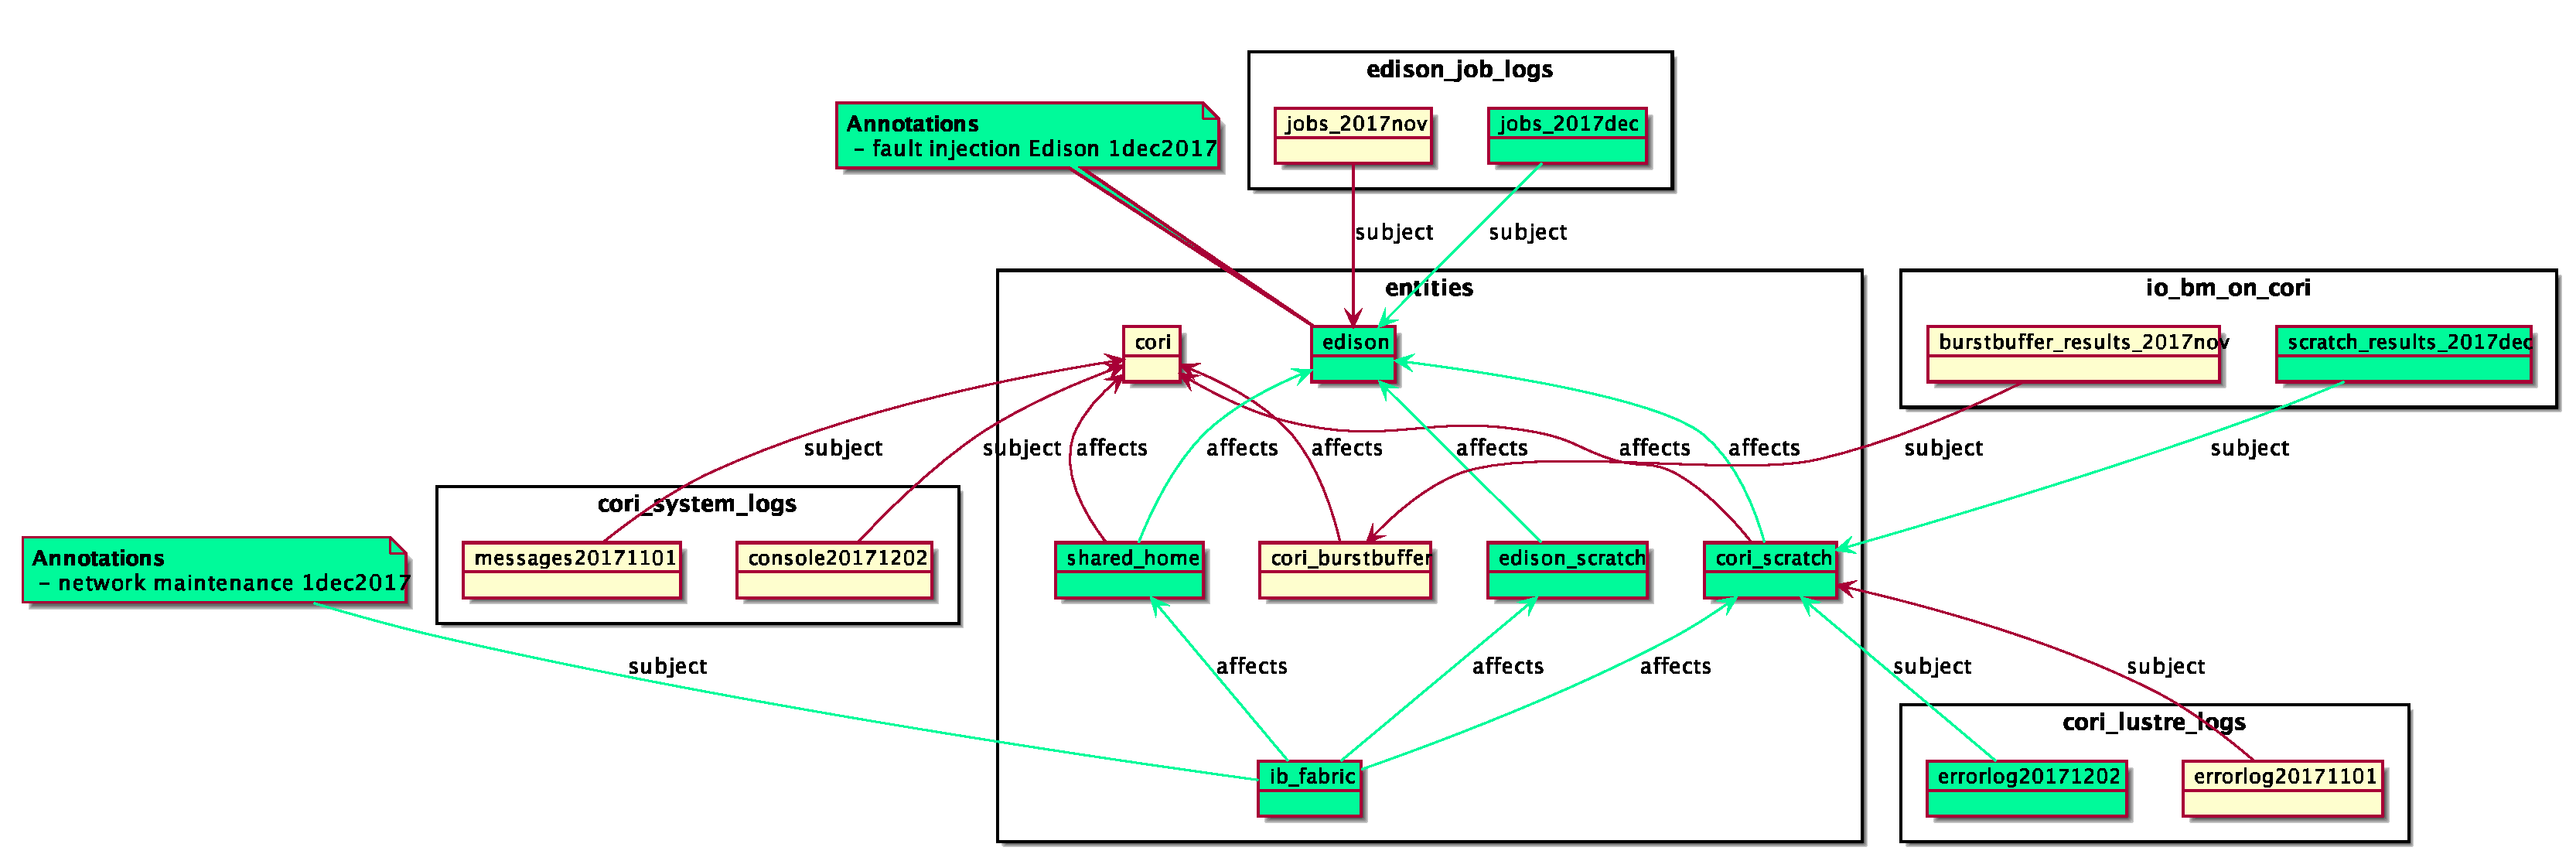
\includegraphics[width=0.9\textwidth]{datasets-example}
%  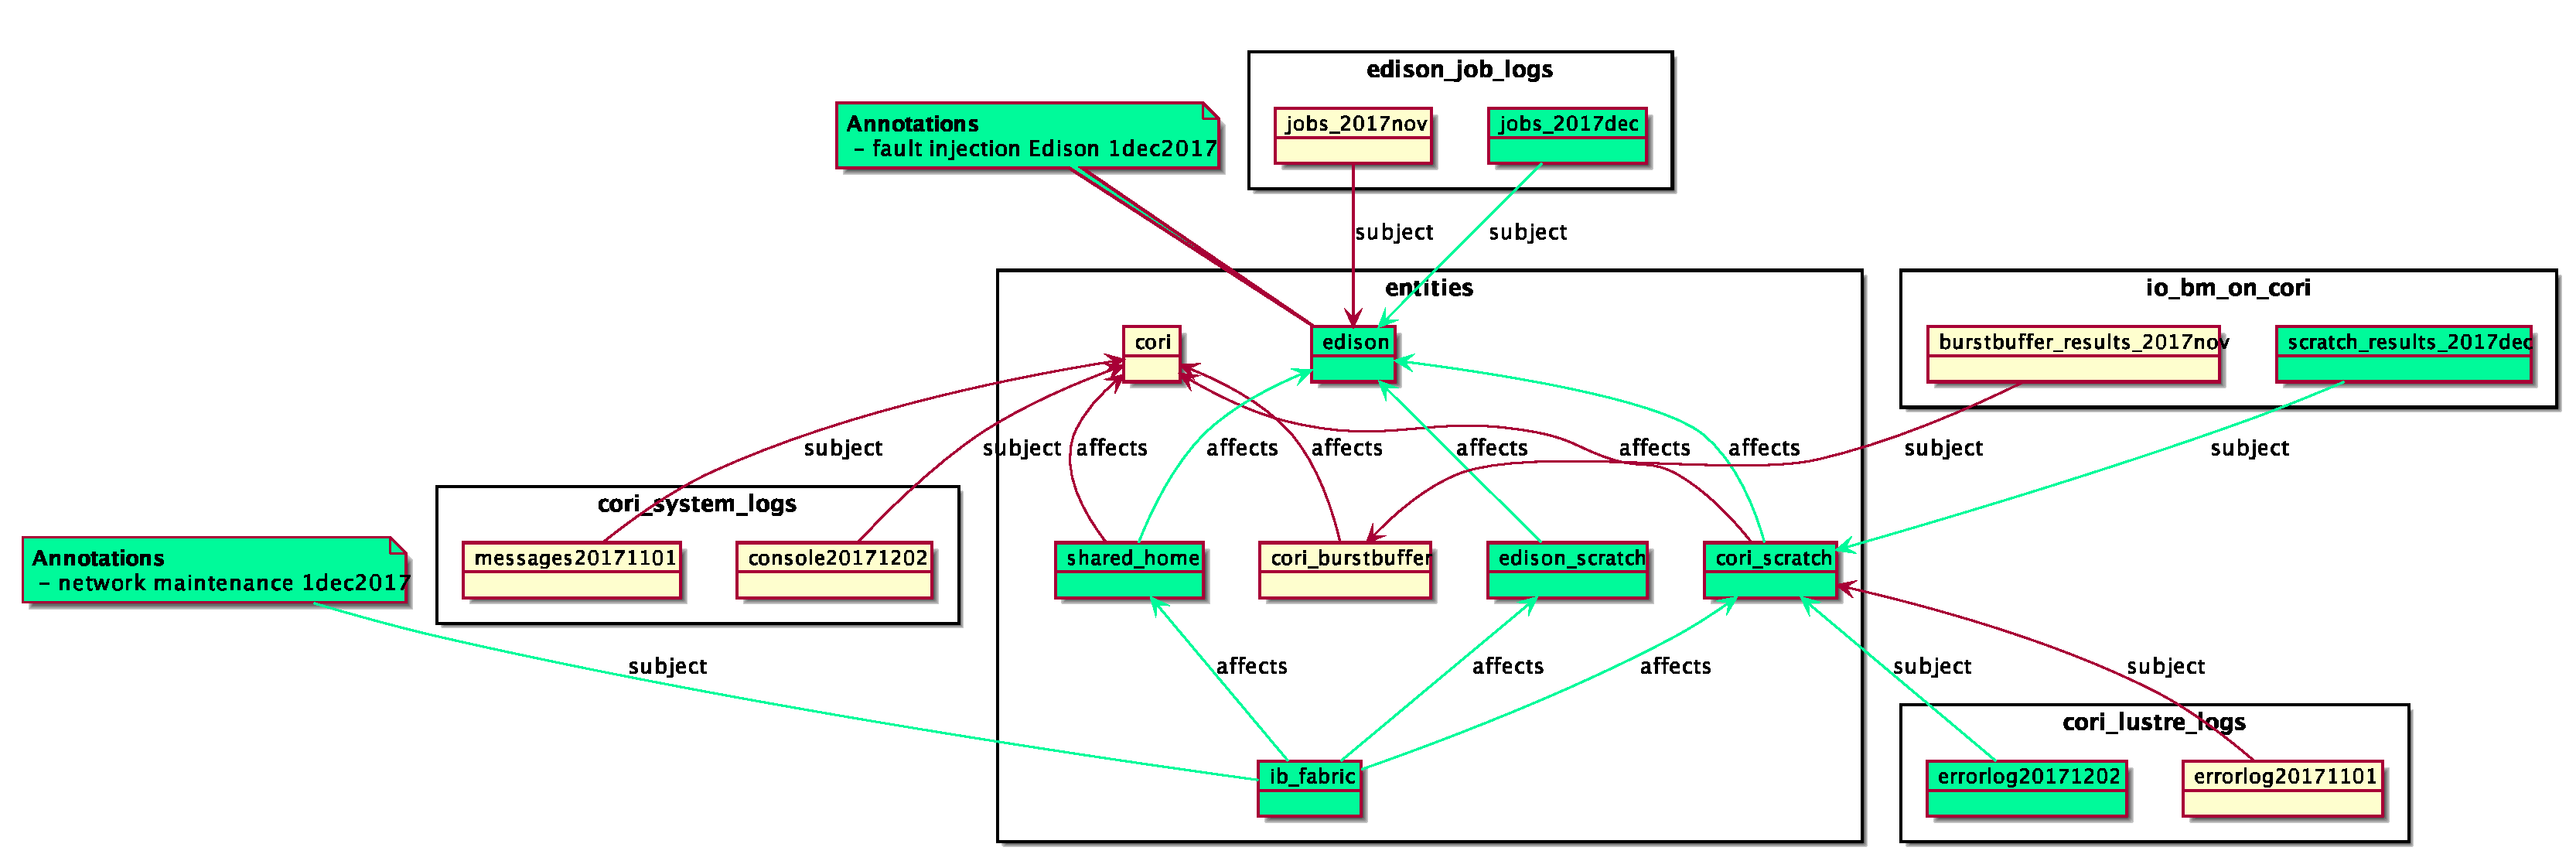
\includegraphics[height=3cm]{datasets-example}
  \caption{Querying a distributed graph from multiple
contributors for logs and annotations related to a particular system at a
particular time.}
\end{figure*}

\section{Contributions of this paper}
We present a solution for annotating log data with human-made observations, and
for publishing and discovering annotations and log data without imposing an
unsustainable burden of effort on either those collecting data or those
analyzing it.

\begin{itemize}
\item We present a mechanism to publish descriptions of collected data
% so as to be
wherby data is easily discoverable with existing linked-data tools, without
reliance on existing knowledge of who is collecting or using which data.
%and requires no heroic effort on the part of either.
By requiring minimal effort we enable a sustainable ecosystem of data collection
and analysis.

\item We present a schema for annotations in which human (or machine-generated)
observations can be published and linked to log data. The schema supports
observations associated with both an imprecise timespan and with specific log
entries; and allows disparate observations of the same subject to be combined. A
set of annotations is a dataset in its own right and can be published and
discovered in the same way.

\item We present tools to help generate, publish, and discover these annotations.
This will enable annotators, data collectors, and researchers to perform typical tasks
and queries without the need to learn the underlying technologies (i.e.,
SQL, RDF and SPARQL).

\item We present case studies demonstrating the use and benefits these on a
a large (Cori) Cray system and a small testbed at different sites.
These tools can support other Cray
sites in sharing and using annotated datasets to better understand and mitigate
faults
%propagation
in Cray systems.
\end{itemize}

\section{Annotation}
Annotations can enable domain experts to provide meaningful information 
(e.g., event descriptions, log entry meanings) required for analysts, without 
domain knowledge, to gain useful insights from otherwise meaningless data.
%Annotations allow those with domain knowledge to describe an event and identify
%relevant log entries so as to be meaningful to analysts without that domain
%knowledge. 
We present an annotation schema allowing human-described events to
be accessed via the same interface as log entries, thus allowing observations
to be overlaid on log entries for investigation of events of interest.

Our schema is a set of SQL tables whose entries describe an event with regards
to timespan, state of the system before and after, and related events. Entries
can be mapped to record-identifiers for specific log types. This enables 
description of events by both approximate timespan and 
%also to call out
specific relevant log entries.

The schema includes provenance information and is designed to support merging of
annotation entries from multiple sources.

\section{Discovery}
The integration of diverse but related information is a motivating case for
linked data and semantic web technologies. It also describes the challenge
faced by researchers investigating resiliency on Cray and other large systems.
Therefore we have based our discovery mechanism on established linked-data
technologies.

We extend the W3C DCAT (Data Catalog) vocabulary to specifically cover log-like
data, including access and format details, and use the ADMS (Asset
Description) and FOAF (Friend-of-a-Friend) vocabularies to describe the subjects
and publishers of monitoring data.

Datasets and catalogs form a queryable, distributed graph of URIs. A site can
publish a catalog of local data with links to a few other catalogs. Local
staff can add links in their local catalog to their own data which then
becomes part of the global graph. Figure 1 illustrates how data added from
disparate sources forms a single graph that can be queried to find all logs
that might have contributed to an event on a specific system (Edison) at a
particular time.

Our annotation schema allows human-made observations to integrate into this
graph, providing both a data point and a starting point for new queries

A key point is that the graph is comprised only of metadata. The log data
itself typically has constraints around security, privacy, or sheer volume.
Data is collected primarily for a specific internal use and the effort required
to clean and publish it for ``the greater good" is generally enough to prevent it
from being published. By asking collectors to publish only metadata we reduce
the publishing effort to a sustainable level.

\section{Putting it all together}
The learning curve for using the underlying SQL and linked data technologies
itself presents an obstacle to publishing and using log data, but most use
cases for publishers, annotators and analysts are based on only a few queries.
To mitigate this obstacle we provide tools that guide users through common
tasks without requiring direct use of SQL or SPARQL. This does not preclude
direct use of the underlying technology by those comfortable with it.

Finally, we present case studies on systems at different sites illustrating the mechanism,
benefit, and general applicability of the tools and schema presented here. Cases include:

\paragraph{User investigation of system events impacting job performance} Application
performance can be impacted by events which are apparent in log data but not exposed to 
users or not apparent to someone without appropriate domain knowledge to interpret the
log data. Our framework enables investigation by users or support staff by exposing 
expert translations of significant occurrences without necessarily exposing logs beyond
their normal security and privacy domain. In addition, the framework enables users to
identify and specify to support staff relevant slices of logs they cannot directly 
access, reducing the effort required by support staff to aid in such questions.

In this example, we show how a user can investigate underlying reasons for and
occurrences of performance variation issues by integrated access of expert annotations 
of CPU throttling events, link degrades, and memory errors which occur in disparate 
Cray logs in conjunction with historic job data.

\paragraph{Administrator event investigation}
The historical state of the system includes not only events captured by the logs, but
human-invoked actions as well, such as DIMM replacement, software upgrades, and cable reseating.
Our annotation system enables labeling and search of both human-defined and system-defined events
in a consistent way, and the return of such events in a format suitable for plotting or additional analysis.

This example shows how the investigation of component faults and resolution can be facilitated by our
framework. Sequences of failures followed by manual resolution action are easily discoverable and visualized
in a timeline. The easy determination of the time between problem onset and resolution is useful for
reporting of the system impact of particular component problems. Finally, long term analysis is used to
detect components (e.g., nodes) which indicate more faults over time, regardless of replacement, which can indicate that
the root cause of problems is environmental (e.g., temperature) rather than component-based.

A related example demonstrates characterization of the impacts of
events which are resolved by the system itself: network failure events which should be resolved by the automatic recalculation
of network routes. Using our framework on production and
fault injection data, we show how the timescales of impact are easily discovered, as well as the discovery
of events for which successful rerouting did not occur. Identification of these occurrences also then facilitates
direction to regions of the logs for more in-depth analysis as to the circumstances of the failure.








